\documentclass{beamer}
\mode<presentation>
\usepackage{amsmath,amssymb,mathtools}
\usepackage{textcomp}
\usepackage{gensymb}
\usepackage{adjustbox}
\usepackage{subcaption}
\usepackage{enumitem}
\usepackage{multicol}
\usepackage{listings}
\usepackage{url}
\usepackage{graphicx} % <-- needed for images
\def\UrlBreaks{\do\/\do-}

\usetheme{Boadilla}
\usecolortheme{lily}
\setbeamertemplate{footline}{
  \leavevmode%
  \hbox{%
  \begin{beamercolorbox}[wd=\paperwidth,ht=2ex,dp=1ex,right]{author in head/foot}%
    \insertframenumber{} / \inserttotalframenumber\hspace*{2ex}
  \end{beamercolorbox}}%
  \vskip0pt%
}
\setbeamertemplate{navigation symbols}{}

\lstset{
  frame=single,
  breaklines=true,
  columns=fullflexible,
  basicstyle=\ttfamily\tiny   % tiny font so code fits
}

\numberwithin{equation}{section}

% ---- your macros ----
\providecommand{\nCr}[2]{\,^{#1}C_{#2}}
\providecommand{\nPr}[2]{\,^{#1}P_{#2}}
\providecommand{\mbf}{\mathbf}
\providecommand{\pr}[1]{\ensuremath{\Pr\left(#1\right)}}
\providecommand{\qfunc}[1]{\ensuremath{Q\left(#1\right)}}
\providecommand{\sbrak}[1]{\ensuremath{{}\left[#1\right]}}
\providecommand{\lsbrak}[1]{\ensuremath{{}\left[#1\right.}}
\providecommand{\rsbrak}[1]{\ensuremath{\left.#1\right]}}
\providecommand{\brak}[1]{\ensuremath{\left(#1\right)}}
\providecommand{\lbrak}[1]{\ensuremath{\left(#1\right.}}
\providecommand{\rbrak}[1]{\ensuremath{\left.#1\right)}}
\providecommand{\cbrak}[1]{\ensuremath{\left\{#1\right\}}}
\providecommand{\lcbrak}[1]{\ensuremath{\left\{#1\right.}}
\providecommand{\rcbrak}[1]{\ensuremath{\left.#1\right\}}}
\theoremstyle{remark}
\newtheorem{rem}{Remark}
\newcommand{\sgn}{\mathop{\mathrm{sgn}}}
\providecommand{\abs}[1]{\left\vert#1\right\vert}
\providecommand{\res}[1]{\Res\displaylimits_{#1}}
\providecommand{\norm}[1]{\lVert#1\rVert}
\providecommand{\mtx}[1]{\mathbf{#1}}
\providecommand{\mean}[1]{E\left[ #1 \right]}
\providecommand{\fourier}{\overset{\mathcal{F}}{ \rightleftharpoons}}
\providecommand{\system}{\overset{\mathcal{H}}{ \longleftrightarrow}}
\providecommand{\dec}[2]{\ensuremath{\overset{#1}{\underset{#2}{\gtrless}}}}
\newcommand{\myvec}[1]{\ensuremath{\begin{pmatrix}#1\end{pmatrix}}}
\newcommand{\mydet}[1]{\ensuremath{\begin{vmatrix}#1\end{vmatrix}}}

\newenvironment{amatrix}[1]{%
  \left(\begin{array}{@{}*{#1}{c}|c@{}}
}{%
  \end{array}\right)
}

\newcommand{\myaugvec}[2]{\ensuremath{\begin{amatrix}{#1}#2\end{amatrix}}}
\let\vec\mathbf
% ---------------------

\title{Matgeo Presentation - Problem 5.2.58}
\author{ee25btech11056 - Suraj.N}

\begin{document}

\begin{frame}
  \titlepage
\end{frame}

\begin{frame}{Problem Statement}

Solve the system of equations
\[
\begin{aligned}
x - y + z &= 4\\
2x + y - 3z &= 0\\
x + y + z &= 2
\end{aligned}
\]
\end{frame}

\begin{frame}{Data}

\begin{table}[h!]
  \centering
  \begin{table}[h!]
    \centering
    \begin{tabular}{|c|c|}
        \hline
        Point & Coordinates \\
        \hline
	    $A$ & $\myvec{1\\-1}$ \\
	    $B$ & $\myvec{-4\\2k}$ \\
	    $C$ & $\myvec{-k\\-5}$ \\
        \hline
    \end{tabular}
    \caption{Vertices of $\triangle ABC$ before substituting $k$}
    \label{tab:triangle_k}
\end{table}

  \caption*{Table : Equations}
  \label{5.2.58}
\end{table}

\end{frame}

\begin{frame}{Solution}

The system of equations in matrix form is :

\begin{align}
  \myvec{1 & -1 & 1\\2 & 1 & -3\\1 & 1 & 1}\myvec{x\\y\\z} &= \myvec{4\\0\\2}
\end{align}

Forming the augmented matrix,

\begin{align}
  \myaugvec{3}{1 & -1 & 1 & 4\\ 2 & 1 & -3 & 0\\1 & 1 & 1 & 2}
\end{align}

Using Gaussian elimination,

\begin{align}
  \myaugvec{3}{1 & -1 & 1 & 4\\ 2 & 1 & -3 & 0\\1 & 1 & 1 & 2}
  \xleftrightarrow[\;R_2 \to R_2 -2R_1\;]{\;R_3 \to R_3 - R_1}
  \myaugvec{3}{1 & -1 & 1 & 4\\0 & 3 & -5 & -8\\0 & 2 & 0 & -2}
\end{align} 

\end{frame}

\begin{frame}{Solution}

\begin{align}
  \myaugvec{3}{1 & -1 & 1 & 4\\0 & 3 & -5 & -8\\0 & 2 & 0 & -2}
  \xleftrightarrow{R_3 \to R_3 -\tfrac{2}{3}R_2}
  \myaugvec{3}{1 & -1 & 1 & 4\\0 & 3 & -5 & -8\\0 & 0 & \tfrac{10}{3} & \tfrac{10}{3}}
\end{align}

Using back substitution we get :

\begin{align}
  \tfrac{10}{3} z &= \tfrac{10}{3}\\ 
  z &= 1\\
  3y - 5z &= -8\\
  3y - 5 &= -8\\
  3y &= -3\\
  y &= -1\\
  x - y + z &= 4\\
  x + 2 &= 4\\
  x &= 2
\end{align}

\end{frame}

\begin{frame}{Solution}

Therefore the solution for the system of equations is : 

\begin{align}
  \myvec{2\\-1\\1}
\end{align}

\end{frame}

\begin{frame}{Plot}

\begin{figure}[h!]
  \centering
  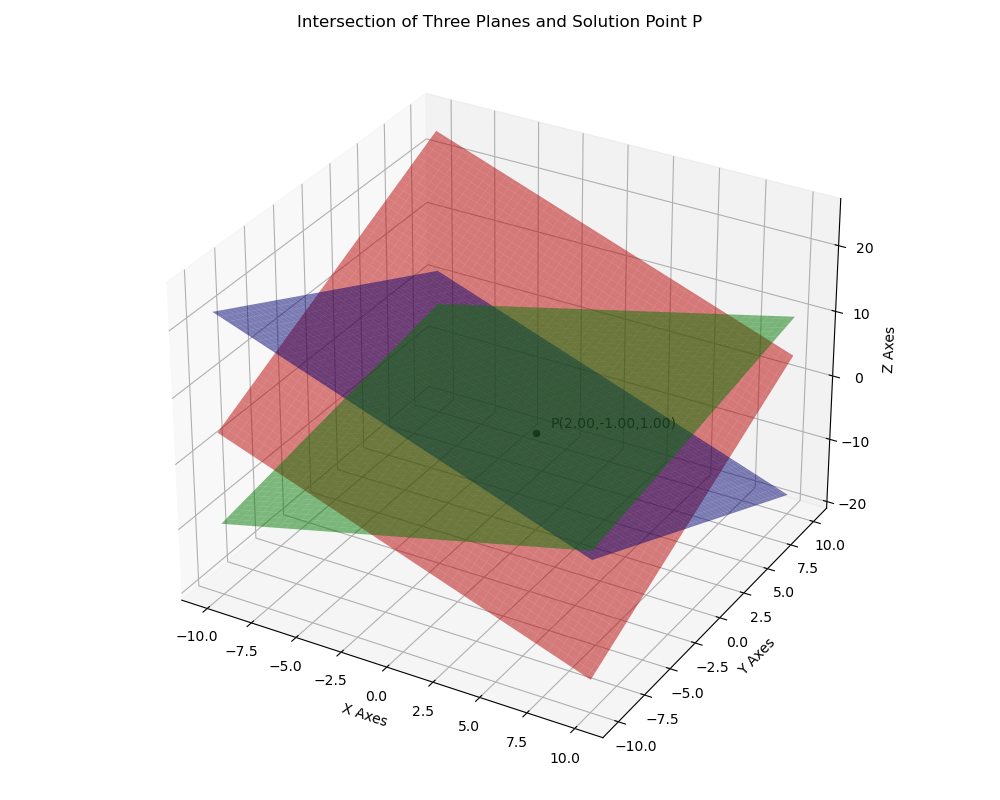
\includegraphics[width=0.8\columnwidth]{figs/solution.png} 
   \caption*{Fig : Planes}
  \label{Fig1}
\end{figure}

\end{frame}



\end{document}
